\documentclass[10pt,a4paper]{article}

\usepackage[margin=18mm]{geometry}

\usepackage[T1]{fontenc}

\usepackage{lmodern,booktabs,longtable,graphicx,pdflscape,hyperref}

\hypersetup{colorlinks=true,urlcolor=blue}

\setlength{\parindent}{0pt}

\setlength{\parskip}{5pt}

\setlength{\emergencystretch}{2em}

\begin{document}

\begin{center}{\Large\bfseries PointSAT checkpoint scaling study --- DRAFT}\end{center}

\section*{Protocol and interpretation}

Five geometric families; the registered number of diverse SAT-only targets per family; one registered native seed per target. Every arm/budget starts afresh from the same frozen target and seed. Native allowances are 10, 30, 60 seconds, not whole-trial wall or CPU budgets. This is a small, deliberately selected, non-IID corpus, not a population success-rate estimate.

The primary endpoint is exact geometric validity of the final saved checkpoint. Any saved valid point set is secondary. For 19 points, printed-coordinate geometric validity is distinct from exact threefold-symmetry reconstruction and from realizing the initial SAT target. For the cap problem, caps are counted in the actual coordinate x direction.

The 19-point arms compare upstream continuous search, v4 continuous search, and v4 split-budget target repair plus warm restart. The last is a compound strategy, not an isolated feedback effect. Paper-family arms use upstream, v6 plain, v6 line, v6 line+pair, and v6 feedback. No time of actual first success is observed or interpolated. Solve-rate differences are not fixed-work kernel speedups.

\textbf{Incomplete snapshot.} Pending targets are not failures; hollow plot points are incomplete. Missing measurements remain unknown. SQL budget-effects and saved-summary snapshots can have slightly different cutoff times while workers run.

The nineteen corpus contains 9 fresh, 11 historical initial sat. All committed fresh targets are considered first, followed by historical initial SAT assignments in frozen source/line order. No coordinate-success or feedback-outcome selection is used. Historical proof-filtered targets are a reused stratum, not all-fresh generation. The known positive-control canonical type is excluded; retained targets satisfy the original CNF and the registered canonical/distance checks. Benchmark checks use the original CNF, not the extra generation cuts.

\section*{Final-checkpoint success counts}

Each cell is valid final outputs / completed trials. The planned count is listed per problem/arm. Missing entries are not measured zeroes.

\begin{center}\small\begin{longtable}{llrrrr}
\toprule
Problem & Arm & Planned & 10 s & 30 s & 60 s \\
\midrule\endhead
symmetry19 & Upstream & 20 & 0 / 12 & 0 / 14 & 0 / 12 \\
symmetry19 & v4 fixed target & 20 & 0 / 12 & 0 / 12 & 0 / 12 \\
symmetry19 & v4 feedback & 20 & 0 / 12 & 0 / 12 & 0 / 12 \\
mixed23 & Upstream & 20 & 0 / 1 & 0 / 1 & 0 / 1 \\
mixed23 & v6 plain & 20 & 0 / 1 & 0 / 1 & 0 / 1 \\
mixed23 & v6 line & 20 & 0 / 1 & 0 / 1 & 0 / 1 \\
mixed23 & v6 line+pair & 20 & 0 / 1 & 0 / 1 & 0 / 1 \\
mixed23 & v6 feedback & 20 & 0 / 1 & 0 / 1 & 0 / 1 \\
holes29 & Upstream & 20 & 0 / 0 & 0 / 0 & 0 / 0 \\
holes29 & v6 plain & 20 & 0 / 0 & 0 / 0 & 0 / 0 \\
holes29 & v6 line & 20 & 0 / 0 & 0 / 0 & 0 / 0 \\
holes29 & v6 line+pair & 20 & 0 / 0 & 0 / 0 & 0 / 0 \\
holes29 & v6 feedback & 20 & 0 / 0 & 0 / 0 & 0 / 0 \\
gons32 & Upstream & 20 & 0 / 0 & 0 / 0 & 0 / 0 \\
gons32 & v6 plain & 20 & 0 / 0 & 0 / 0 & 0 / 0 \\
gons32 & v6 line & 20 & 0 / 0 & 0 / 0 & 0 / 0 \\
gons32 & v6 line+pair & 20 & 0 / 0 & 0 / 0 & 0 / 0 \\
gons32 & v6 feedback & 20 & 0 / 0 & 0 / 0 & 0 / 0 \\
caps26 & Upstream & 20 & 0 / 0 & 0 / 0 & 0 / 0 \\
caps26 & v6 plain & 20 & 0 / 0 & 0 / 0 & 0 / 0 \\
caps26 & v6 line & 20 & 0 / 0 & 0 / 0 & 0 / 0 \\
caps26 & v6 line+pair & 20 & 0 / 0 & 0 / 0 & 0 / 0 \\
caps26 & v6 feedback & 20 & 0 / 0 & 0 / 0 & 0 / 0 \\
\bottomrule\end{longtable}\end{center}


\clearpage\begin{landscape}

\section*{Checkpoint scaling and actual residuals}

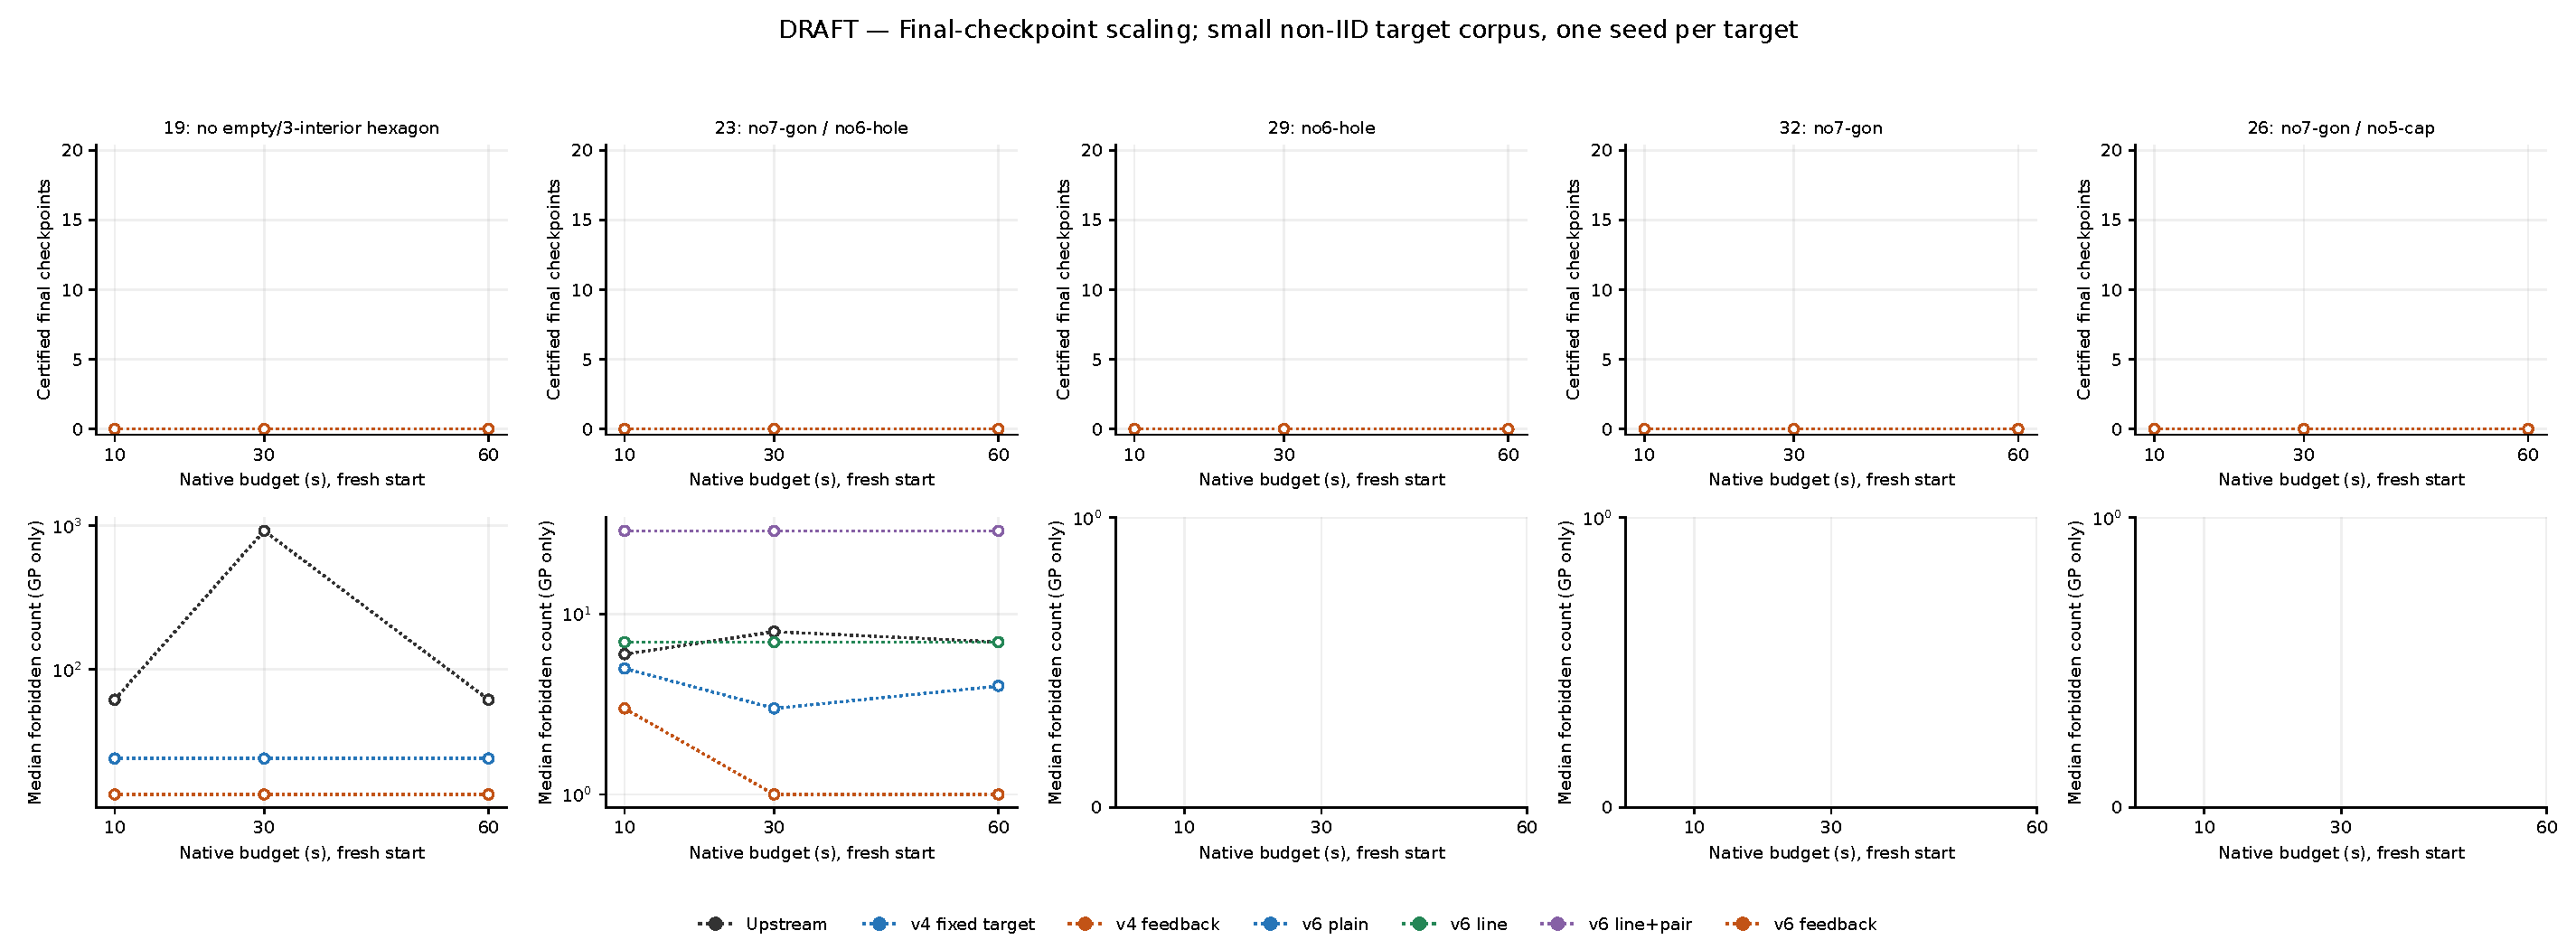
\includegraphics[width=\linewidth]{checkpoints.pdf}

Top: valid final checkpoints. Bottom: median actual forbidden polygon/cap count among general-position (GP) finals only. GP denominators and target-orientation errors are in README.md and report.json. Scales differ between families. Dotted connections describe independent budget starts, not continuous survival curves. Coincident arm values can overlap.

\end{landscape}\clearpage

\section*{Paired effect of more native time}

Gains/losses compare validity of the same target and seed. The residual delta is higher-budget minus lower-budget forbidden count, then a median across paired GP targets. It is not the difference of group medians. Both endpoints need a hash/content-checked stored audit certificate for inclusion in residual changes. Negative deltas are improvements; longer runs can lose final-checkpoint validity.

\begin{center}\small\begin{longtable}{llrrrrrr}
\toprule
Problem & Arm & Pairs & 10$\to$30 G/L & Delta (GP) & Pairs & 30$\to$60 G/L & Delta (GP) \\
\midrule\endhead
symmetry19 & Upstream & 12 & 0/0 & 0.00 (12) & 12 & 0/0 & 0.00 (12) \\
symmetry19 & v4 fixed target & 12 & 0/0 & 0.00 (12) & 12 & 0/0 & 0.00 (12) \\
symmetry19 & v4 feedback & 12 & 0/0 & 0.00 (12) & 12 & 0/0 & 0.00 (12) \\
caps26 & Upstream & 0 & 0/0 & -- (0) & 0 & 0/0 & -- (0) \\
caps26 & v6 plain & 0 & 0/0 & -- (0) & 0 & 0/0 & -- (0) \\
caps26 & v6 line & 0 & 0/0 & -- (0) & 0 & 0/0 & -- (0) \\
caps26 & v6 line+pair & 0 & 0/0 & -- (0) & 0 & 0/0 & -- (0) \\
caps26 & v6 feedback & 0 & 0/0 & -- (0) & 0 & 0/0 & -- (0) \\
gons32 & Upstream & 0 & 0/0 & -- (0) & 0 & 0/0 & -- (0) \\
gons32 & v6 plain & 0 & 0/0 & -- (0) & 0 & 0/0 & -- (0) \\
gons32 & v6 line & 0 & 0/0 & -- (0) & 0 & 0/0 & -- (0) \\
gons32 & v6 line+pair & 0 & 0/0 & -- (0) & 0 & 0/0 & -- (0) \\
gons32 & v6 feedback & 0 & 0/0 & -- (0) & 0 & 0/0 & -- (0) \\
holes29 & Upstream & 0 & 0/0 & -- (0) & 0 & 0/0 & -- (0) \\
holes29 & v6 plain & 0 & 0/0 & -- (0) & 0 & 0/0 & -- (0) \\
holes29 & v6 line & 0 & 0/0 & -- (0) & 0 & 0/0 & -- (0) \\
holes29 & v6 line+pair & 0 & 0/0 & -- (0) & 0 & 0/0 & -- (0) \\
holes29 & v6 feedback & 0 & 0/0 & -- (0) & 0 & 0/0 & -- (0) \\
mixed23 & Upstream & 1 & 0/0 & 2 (1) & 1 & 0/0 & -1 (1) \\
mixed23 & v6 plain & 1 & 0/0 & -2 (1) & 1 & 0/0 & 1 (1) \\
mixed23 & v6 line & 1 & 0/0 & 0 (1) & 1 & 0/0 & 0 (1) \\
mixed23 & v6 line+pair & 1 & 0/0 & 0 (1) & 1 & 0/0 & 0 (1) \\
mixed23 & v6 feedback & 1 & 0/0 & -2 (1) & 1 & 0/0 & 0 (1) \\
\bottomrule\end{longtable}\end{center}


All registered budget comparisons, fewer/same/more counts, missing pair sides, non-GP/audit exclusions, and secondary orientation-error changes are preserved in report.json and the Markdown report.

\clearpage

\section*{Compute accounting}

CPU seconds measure processor consumption; summed worker-wall seconds are not elapsed calendar time. Native allowance excludes SAT feedback, initial flippability/preparation, and exact audits. Worker CPU beyond native includes initialization and unclassified work; it is not a pure SAT timer.

\begin{center}\small\begin{longtable}{llrr}
\toprule
Study & Component & CPU seconds & Worker wall seconds \\
\midrule\endhead
nineteen & Native & 3652.73 & 3660.57 \\
nineteen & Other/unclassified search worker & 706.44 & -- \\
nineteen & Exact audits & 32.40 & 34.59 \\
nineteen & Shared preparation & 268.83 & 270.09 \\
nineteen & Fresh corpus generation & 1798.74 & 1800.07 \\
nineteen & Combined-corpus validation & 12.54 & 14.38 \\
nineteen & Combine controller & 1.50 & -- \\
paper & Native & 498.32 & 500.05 \\
paper & Other/unclassified search worker & 5.14 & -- \\
paper & Exact audits & 4.93 & 5.24 \\
paper & Shared preparation & 1.13 & 1.15 \\
paper & Fresh corpus generation & -- & -- \\
paper & Combined-corpus validation & -- & -- \\
paper & Combine controller & -- & -- \\
\bottomrule\end{longtable}\end{center}


Shared preparation and corpus costs are counted once, not per arm/budget. Fresh-generation CPU and combined-corpus revalidation are separate. Historical generation sunk costs are not attributed to this batch. Combine wall includes its controller; do not add it again to child wall. Unknown CPU stays unknown; wall time is never substituted. Completed-summary costs and all-attempt totals are separate views and must not be added together.

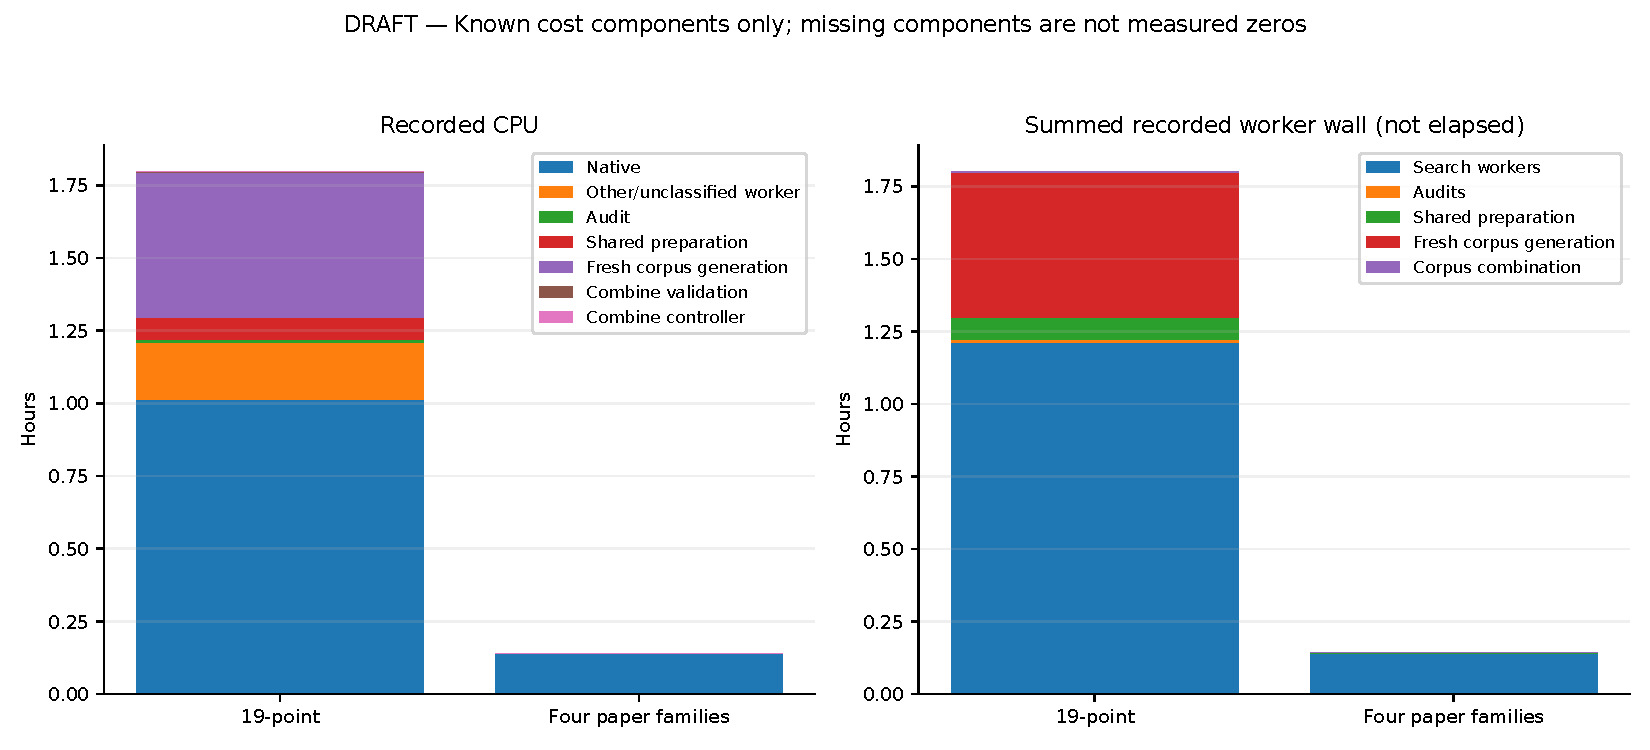
\includegraphics[width=\linewidth]{costs.pdf}

\section*{Errors and censoring}

nineteen: summary complete=False; persisted attempts=112, incomplete attempts=2, external interruptions=2, overhead watchdogs=0, audit watchdogs=0, forced native kills=0.

Recorded statuses: \{"FINISHED": 110, "INTERRUPTED": 2\}.

paper: summary complete=False; persisted attempts=15, incomplete attempts=0, external interruptions=0, overhead watchdogs=0, audit watchdogs=0, forced native kills=0.

Recorded statuses: \{"FINISHED": 15\}.

Ordinary native-budget termination is expected, not an operational error. Failed/missing certificates are not impossibility proofs. Interrupted/inflight work remains separately censored; abrupt termination may leave unrecorded CPU. The machine-readable ledger retains retries, errors, and cost-field coverage.

\section*{Separate positive control}

This is one known realizable type, excluded from the diverse target corpus. Cold-start results are a pipeline sanity check, not a representative solve-rate estimate or part of the diverse-target denominators.

\begin{center}\small\begin{longtable}{lrrrr}
\toprule
Arm & Geometry valid & Native CPU s & Native wall s & Target errors \\
\midrule\endhead
Upstream & True & 1.66 & 1.67 & 3 \\
v4 fixed target & True & 1.46 & 1.52 & 6 \\
\bottomrule\end{longtable}\end{center}


\section*{Provenance and reproduction}

This PDF, README.md, report.json, scaling-report.tex, and the vector/PNG figures form one read-only report snapshot. The JSON records full input/output hashes, frozen corpus provenance, raw-attempt diagnostics, and paired effects. No searches or geometry audits are run during report generation. Earlier reports remain untouched.

nineteen registration: \url{/home/andrew/PointSAT/benchmarks/compare19_scaling_20260907/registration.json}\\{\footnotesize\texttt{867cdb70c0622ab441ec830f92c2cb9eec7802738ca81306cf37a51faf420fe6}}

paper registration: \url{/home/andrew/PointSAT/benchmarks/paper_scaling_20260907/registration.json}\\{\footnotesize\texttt{802ca2d1f810f6b6acf39bf29e1840a91db6c3672d056986ce92471502d4580c}}

Machine/environment snapshot: {\small\url{/home/andrew/PointSAT/benchmarks/scaling_machine_20260907.json}}. This does not imply exclusive ownership of every machine core.

Positive-control source: {\small\url{/home/andrew/PointSAT/benchmarks/compare19_positive_control_20260907/result.json}}

\end{document}

